\subparagraph{Задание 4.6 (1)}

\textbf{Условие}:
Загрузить программу в отладчик (td \path{d:\asm\lab2}). Какими способами это можно сделать? Отразить способы в отчете.

\textbf{Решение}:

\begin{lstlisting}[language=Terminal]
    $ C:\td\td.exe lab2
\end{lstlisting}

\begin{figure}[!htp]
    \centering
    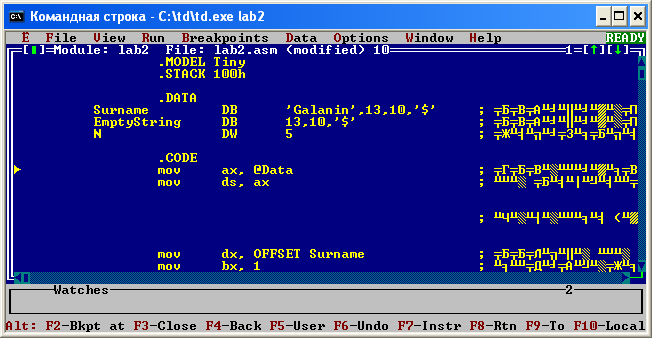
\includegraphics[width=11.2cm]{../_INCLUDES/td.png}
    \caption{td lab2}
\end{figure}

Загрузить программу в отладчик можно 

\begin{enumerate}
    \item Прописав команду \verb|$ td path\to\file|
    \item В программе Turbo Debugger нажать F10. Нажать влево, выбрав пункт File. Нажать Enter. Выбираем пункт Open.
\end{enumerate}

\begin{figure}[!htp]
    \centering
    \begin{minipage}{0.48\textwidth}
        \centering
        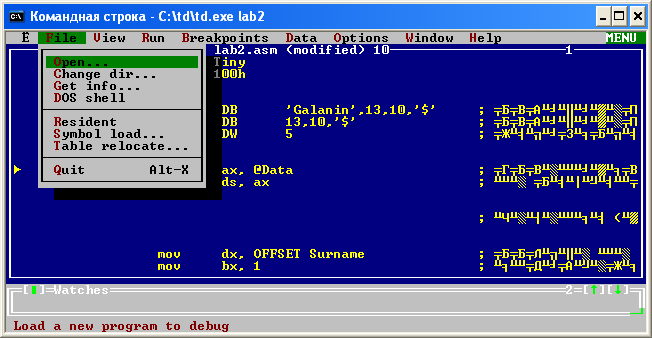
\includegraphics[width=.98\linewidth]
            {../_INCLUDES/task-4-6-1/td-file.png}
        \caption{td >FILE}
    \end{minipage}
    \begin {minipage}{0.48\textwidth}
        \centering
        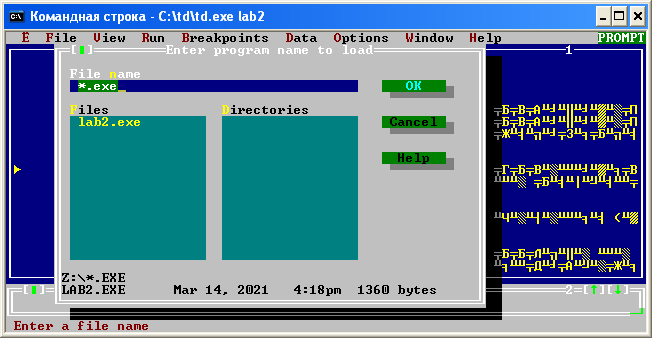
\includegraphics[width=.98\linewidth]
            {../_INCLUDES/task-4-6-1/td-file-open.png}
        \caption{td >FILE>OPEN}
    \end{minipage}
\end{figure}
